\chapter{Application Domain}
This chapter aims to define the required functionality of both the server and the client side of the solution. Furthermore, this chapter describes which types of persons could be using the solution. 


\section{Interaction Design}
\subsection{PACT - designing for people}\label{pact}
\frnote{ret mig}
When designing an interactive system it is important to think about the people using it. The people are a part of the interactive system and therefore it is important to make sure that the design fit the people. In \cite{benyon2013designing} the acronym PACT is presented as a framework for thinking about design situations. To help with the design being human centered the designer need to understand the 4 letters in the acronym: It is important to understand the different kind of people using the system since they have different prerequisite for using a system. The activities that people want to undertake. When thinking about the context the designer need to think about the location it will be used. Lastly the designer should consider the features of interactive technologies and how to use them in the design.

\begin{figure}
  \centering
  \includegraphics[width=0.5\linewidth]{pact-overview.png}
  \caption{The relationships between activities, contexts, people and technologies in PACT. From \cite{benyon2013designing}}
  \label{fig:pact-overview}
\end{figure}

It is also important to understand the relationship between activities and technologies. \Cref{fig:pact-overview} shows how the activities people are doing will influence the requirements for teknologi. This will create new technology that will change to activities people will be doing with the technologi.

It is the variety of requirements that is found during the PACT analysis that can make designing systems difficult. Therefore, they will be conducted a study of the element in PACT.


\subsection{People}
\label{sub:pact_people}

The system is used by people who go to bar-like environments, and are possibly intoxicated. At bar-like environments, music is central to the atmosphere, and a lot of people are interested in having their music tastes accommodated. Different people exhibit different behaviour in these social contexts, some may clique together when using a social system and some may be afraid of stigmas when using it. To use the system, a smartphone is required, and some people may be unable or afraid to use their smartphone.

\subsection{Activities}
\label{sub:pact_activities}

Usage of the system requires the user to interact with their smartphone or similar device. Firstly the user must install the application on their device and sign in using their Facebook or Google account. When the user has signed in to the application, they will either have to go to the voting screen or request screen. When in the voting screen, the user can press an upvote button or downvote button for each song in the playlist. In the request screen, users can browse the available library, find a song they like and add it to the playlist.

\subsection{Context}
\label{sub:pact_context}

This system can be used at places where many people wants to listen to music, but does not have an efficient method of determining which songs to listen to.

A dark environment with a lot of noise is common in bars/pubs. As people are often dancing in this environment, active use of smartphones is not recommended. Also, usage of smartphones in these kind of environments often cause anti-social behavior.

\subsection{Technologies}
\label{sub:pact_technologies}

The system runs on a host computer with an audio system connected and a business license for Spotify. This host computer is located at the installation site. 

For users to operate this system a smartphone with internet connection and adequate battery life is required. Login to the system requires a Facebook/Google account.

When designing the system, different smartphones and their characteristics have to be considered.


\subsection{Persona}
\frnote{ret}
The people that use a system can be represented by personas. This is done in order to ensure the PACT elements are centered in the design process\kanote{Hvad menes der her?}. Personas are general profiles of different types of users. A persona is a concrete representation of a fictitious person. Personas help the designer by having a specific end user in mind, preventing them designing the system for themselves. Personas are developed through the understanding process and through undertaking a PACT analysis. A part of the persona is a short story of the person trying to achieve a goal using the system in a specific context~\cite{benyon2013designing}.

As part of this project, a persona was made, based on the interviews which were conducted.%\cref{interviewbruger}.
This is Camilla, an average user of the system.

\subsubsection{Camilla}
\begin{figure} [h]
  \centering
  \includegraphics[]{Images/average.jpg}
  \caption{Picture associated with the persona \enquote{Camilla}. Copyright the Face Research Lab. Used with permission.}
  \label{fig:camilla}
\end{figure}
\noindent\textbf{Basic information}
\begin{itemize}
\item 25 years old
\item Medical student
\item Employed in an elderly care center
\item In a relationship with Keith
\item She loves meeting new people
\item When going out she likes to visit small places that allow socialisation
\item Volunteered in Red Cross Uganda
\end{itemize}

It is Friday afternoon and Camilla is planning to meet some of her fellow students at a bar. Camilla and her friends get together after they are finished at school and go to a café to grab a sandwich. After dinner, Camilla takes out her smartphone and checks openPlaylist. Camilla can see that some of her favourite songs are being played at White Hart, and they agree to go there. Upon arriving Camilla checks in via the application. She immediately notices on the screen behind the bar that the queue is filled with songs she dislikes. She now uses the application to request and upvote other songs that she would like to be played. Some other people at White Hart agree on Camilla's choices and they too upvote these songs. On the screen in the bar Camilla can see some of the other people that upvotes her songs and later in the evening she meets them and they talk about all the nice music they have in common. Camilla and her new and old friends party all night long and drink a lot of beer.

\section{Use Cases}\label{usecase}
\subsection{Actors}
There are two actors of this system; an administrator which could be a
bartender or a bar owner in charge of the music, and a guest wanting
to request and affect the music being played at the venue. Further information about these actors are presented in the below tables for respectively administrators and guests. Based on these actors, actor tables and usage diagrams has been made, see \cref{tab:actorTable,fig:UsageAdmin,fig:UsageUser}. These describe the possible actions each actor can take in the system.

\begin{table}
\centering
\begin{tabular}{lcc}
\hline
                   & \multicolumn{1}{l}{\textbf{Actor}} & \multicolumn{1}{l}{} \\
\textbf{Use case}  & Administrator                      & Customer             \\ \hline
play music         & \checkmark                         &                      \\
stop music         & \checkmark                         &                      \\
next track         & \checkmark                         &                      \\
add restriction    & \checkmark                         &                      \\
remove restriction & \checkmark                         &                      \\
check out          &                                    & \checkmark           \\
check in at venue  &                                    & \checkmark           \\
vote               &                                    & \checkmark           \\
cancel vote        &                                    & \checkmark           \\ \hline
\end{tabular}
\caption{Actor table for the project}\label{tab:actorTable}
\end{table}

\actortable{Administrator}{
    \textbf{Purpose:} A person that protects the interests of the venue and is responsible for the music. He or she wants to be able to have control over the system, what kind and in which order music is being enqueued and what is currently playing.

    \textbf{Characteristics:} Has a preference or a theme of music that the individual is following, set by the organisation or the individual itself. Works at the venue and has a reasonable high technical level or the ability and motivation to be taught the use of the system.

    \textbf{Possible usage:} Administrator 1 is very open minded for all requests and votes from users and only sets the bare minimum restrictions to maintain the theme of the venue.

		Administrator 2 completely controls the playlist by adding, removing and rearranging tracks to completely fit the venue's preferences and what is played. He is very restrictive and only accepts requests and votes that he agrees with.

		Add and remove restrictions, play, pause and stop music, play next track and add, remove and rearrange tracks on the playlist.\\\\
		Diagram of possible usage, see \cref{fig:UsageAdmin}.
}

\begin{figure}
  \centering
  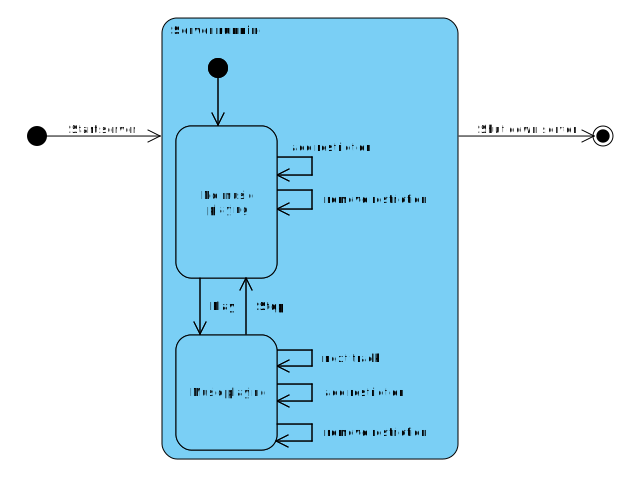
\includegraphics[width=1.1\textwidth]{Images/UsageAdmin.pdf}
  \caption{Usage for a administrator}\label{fig:UsageAdmin}
\end{figure}

\actortable{Guest}{
    \textbf{Purpose:} Wants to influence the playlist and listen to preferred tracks at a venue.

    \textbf{Characteristics:} Has a music preference possibly different from the administrator and/or the specific theme at the specific venue. Varying technical level but with the ability to use his or her smartphone.

    \textbf{Possible usage:} Guest 1 only requests tracks to the playlist but rarely votes on other users tracks.

		Guest 2 only votes on tracks and does not use the feature of requesting tracks.

		A user has the ability to check in and out of a venue, vote and revote for track and cancel their vote.\\\\
		Diagram of possible usage, see \cref{fig:UsageUser}.
}
\begin{figure}
  \centering
  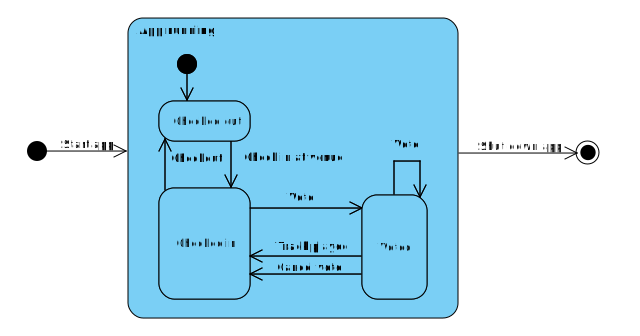
\includegraphics[width=1.1\linewidth]{Images/UsageUser.pdf}
  \caption{Usage for a guest}\label{fig:UsageUser}
\end{figure}


\section{Functions}
As part of the analasys of the application domain an analysis of the functions are needed.
\begin{table}[h]
\begin{tabular}{lll}
\hline
\multicolumn{3}{c}{\textbf{Social music playing}} \\ \hline
Filter                         & Medium & Compute \\
Create filter                  & Simple & Update  \\
Read filter                    & Simple & Read    \\
Update filter                  & Simple & Update  \\
Delete filter                  & Simple & Update  \\
Get current playlist           & Simple & Read    \\
Change song votes              & Simple & Update  \\
Play something on the speakers & Medium & Signal  \\
Change playing state           & Medium & Update  \\
Song vote                      & Medium & Update  \\
Get next song                  & Medium & Compute \\
Noget med søg                  &        &         \\ \hline
\end{tabular}
\end{table}
